
\textbf{一份按「判据能不能被独立重跑」组织的研究（2024-10 — 2026-11）}


\begin{quote}\small
\textbf{数据快照}：2026-11-09 ｜ \textbf{来源}：22 份（14 份基准仓库原文 + 8 篇谱系论文）｜ \textbf{来源时间跨度}：2024-10 至 2026-11 ｜ \textbf{主张}：15 条 ｜ \textbf{证据}：62 条（高置信 13 条）

\end{quote}

\begin{abstract}

2024 年 10 月，MLE-bench 把 75 个 Kaggle 竞赛摆到 agent 面前，判据是「拿到奖牌的比例」。此后两年，这一族换了三次对象：RE-Bench 换成开放式研究工程，PostTrainBench 换成后训练一个模型，RSI-Inference Bench 换成改一个生产推理引擎。每一次换对象，判据都得重造一次。


本文要回答的问题比「它们有多强」更窄也更硬：\textbf{这一族基准的判别力从哪里来，它又在哪些地方已经到底。}


本文核对了 2024 年 10 月至 2026 年 11 月的 22 份材料，其中 14 份是 RSI-Inference Bench 仓库的原文（它没有论文——README 徽章写 \texttt{Paper: coming soon}，CITATION.cff 只有一条指向仓库本身的 \texttt{@misc}）{\scriptsize\texttt{[c-\hspace{0pt}retrieval-\hspace{0pt}gap]}}。核心贡献有四。


\textbf{第一，判据形状是一个梯度，不是三种难度。} RSI-Inference Bench 的 37 题里，Day-0 Model Support 10 题用二元判据（起不起来），Inference Optimization 20 题与 Bug Fix 7 题用连续判据（几何平均加速比）{\scriptsize\texttt{[c-\hspace{0pt}three-\hspace{0pt}tracks]}}。二元判据的可自动化程度最高，因为它不需要任何基线——只要能起服务就算过。这个差别解释了为什么同一批 agent 在两条赛道上的分数差 1.4 倍{\scriptsize\texttt{[c-\hspace{0pt}oracle-\hspace{0pt}exceeded]}}。


\textbf{第二，这道基准的天花板是一张分布，不是一个标量。} 最好的 agent 在 day-0 的 pass@1 是 0.2667，但这个数字的真实形状是「10 题里 5 题有人通过过、5 题全场零通过」{\scriptsize\texttt{[c-\hspace{0pt}ceiling-\hspace{0pt}is-\hspace{0pt}clustered]}}。15 个 agent 乘 10 题共 412 次尝试，只有 23 次全通过，且只有 6 个 agent 有过任何一次（见 图 3）。把这条分布压成一个标量，会丢掉唯一可行动的结论。


\textbf{第三，失败主要是「差一点」。} 同一个 agent 在同一批评测里，fail-to-pass 检查项通过率是 0.9006，而 pass@1 是 0.2667{\scriptsize\texttt{[c-\hspace{0pt}near-\hspace{0pt}miss-\hspace{0pt}gap]}}。也就是说它已经把九成的检查项做对，却因为剩下一成拿不到分。这不是能力的失败，是判据形状的选择——而基准作者是明确选择的（\texttt{A partial pass counts as a failure}）。


\textbf{第四，名字里有 RSI，但循环没闭合——缺的那一段正是「谁来判」。} 这一族已经能改进模型（PostTrainBench 系）与引擎（RSI-Inference Bench），但评测装置本身仍由人在循环外持有：没有一篇让 agent 去改「谁判它对」{\scriptsize\texttt{[c-\hspace{0pt}rsi-\hspace{0pt}not-\hspace{0pt}closed]}}。所有方法侧的进展——DataTree、Experiment OS、轨迹微调——都在把分数做高，没有一条在动判据{\scriptsize\texttt{[c-\hspace{0pt}method-\hspace{0pt}not-\hspace{0pt}judgment]}}。


\textbf{结论：这一族基准的判别力确实来自「判据能不能被独立重跑」，而这也正是它的天花板。} 能独立重跑的判据（起不起得来、快多少倍）已经被工程化到可批量执行，代价是每道题都要能重建环境{\scriptsize\texttt{[c-\hspace{0pt}apparatus-\hspace{0pt}cost]}}；而「这样改对不对」这类不能独立重跑的判据，至今没有一篇把它形式化。


\textbf{关键词}：ML 工程基准；day-0 模型支持；推理引擎；判据形状；验证装置；递归自我改进


\end{abstract}
\section{引言：一个没有论文的基准，和一整族被漏掉的装置}

\subsection{起点是一个检索失败}

2026 年 11 月，一份关于推理优化的综述被问到：RSI-Inference Bench 调研过吗。


查了一遍：没有。不是漏读——是\textbf{检索面不重叠}。那份综述的 57 条来源 100\% 来自 arXiv，而 RSI-Inference Bench 的引用形式是 \texttt{@misc} 指向一个 GitHub 仓库，arXiv 上不存在可召回的条目{\scriptsize\texttt{[c-\hspace{0pt}retrieval-\hspace{0pt}gap]}}。再往下查，整族都不在：MLE-bench、RE-Bench、PostTrainBench、DataMaster、RSI-Master、RSI-Dojo，一篇都没有。


这件事本身就是本文的第一个发现。\textbf{一个只用 arXiv 检索式的流程，会稳定地漏掉「以可执行环境为交付物」的一整族基准，而且漏得毫无声响}——因为校验器只检查「引用了的存不存在」，从不检查「该有的有没有」。


\subsection{本文要检验的假设}

本文的假设只有一句：


\begin{quote}\small
这一族基准的判别力不来自任务难度，而来自\textbf{判据能不能被独立重跑}。

\end{quote}

若成立，则这一族的方法学创新应集中在验证装置（独立 verifier、pinned commit、离线、隐藏测试、guard 工作负载）而不是搜索算法；且凡是判据不能独立重跑的环节，就应当是这一族至今没做出来的环节。


第 3 章给出验证装置的逐条拆解，第 7 章用方法侧的全部进展对它做一次反证，第 8 章给出它失效的位置。


\subsection{纳入标准与数据来源}

\begin{itemize}
  \item \textbf{时间}：2024-10 至 2026-11（最早为 MLE-bench，2024-10-09）
  \item \textbf{锚点}：RSI-Inference Bench 仓库的 14 份原文（README、CITATION、ACKNOWLEDGEMENTS、4 份任务说明书、4 份 task.toml、pier README、leaderboard 原始快照）
  \item \textbf{谱系}：8 篇 arXiv 论文，按「同一族评测装置」纳入
  \item \textbf{排除}：只讲推理优化技术而不含评测装置的（已由另外三篇归档处理）
\end{itemize}

\sym{⚠}{} \textbf{三个必须声明的局限}：


\begin{enumerate}
  \item \textbf{锚点没有论文。} 方法学本该由论文承担，现在只能从 README 的图注与 task.toml 反推。这是全篇最脆的一处。
  \item \textbf{leaderboard 是滚动快照。} 本文用的是 \texttt{2026-10-25T2208Z} 那一版（15 个 agent、555 条计分结果），所有排名陈述都绑定它。
  \item \textbf{本文没有跑任何实验。} 全部数字二手，但每一条都能点回仓库原文或 arXiv 全文。
\end{enumerate}

\section{三条赛道，三种判据形状}

\subsection{一个模型在引擎里的一生}

RSI-Inference Bench 的组织方式不是按难度分级，而是按\textbf{时间}：它跟着一个模型走完它在生产引擎里的一生——被支持、被优化、被修{\scriptsize\texttt{[c-\hspace{0pt}three-\hspace{0pt}tracks]}}。



\begin{table*}[t]
\centering
\footnotesize
\setlength{\tabcolsep}{4pt}
\label{tab:1}
\begin{tabular}{lrlll}
\toprule
赛道 & 题数 & 目标 & 判据 & 部分通过怎么算 \\
\midrule
Day-0 Model Support & 10 & 把新模型服务起来 & pass@1（全通过次数 / 尝试次数） & 按失败计 \\
Inference Optimization & 20 & 更快 & 几何平均加速比 & 正确性不过记 1.00× \\
Bug Fix & 7 & 找到并修掉一个性能回归 & 几何平均加速比 & 同上，另有 guard 形状 \\
\bottomrule
\end{tabular}
\end{table*}

题库 37 题，引擎分布 vLLM 20 / SGLang 17，加速器分布 B200 20 / H100 17，每题 1 至 8 张卡{\scriptsize\texttt{[c-\hspace{0pt}three-\hspace{0pt}tracks]}}。


\begin{figure*}[t]
\centering
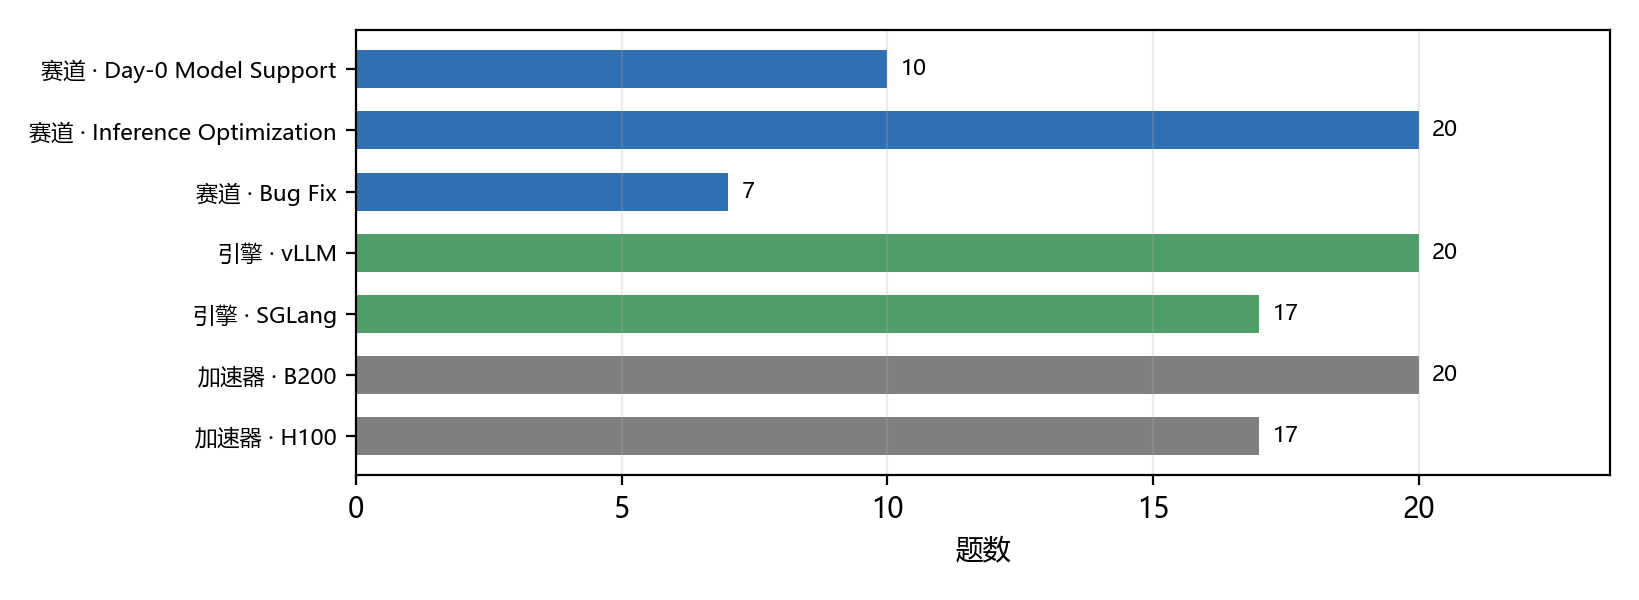
\includegraphics[width=0.86\textwidth]{../figures/fig1_compose.png}
\caption{图 1　题库构成。三个切面（赛道、引擎、加速器）各自加总为 37，用颜色区分——}
\label{fig:1}
\end{figure*}
它们是对同一批题目的三种划分，不是三个可比的量。*


\subsection{二元与连续：不是难度差别，是分母差别}

三条赛道的判据形状差别，说到底是一个分母问题。


Day-0 的 pass@1 分母是\textbf{尝试次数}：10 题各跑 3 次就算 30 次，通过几次除以几次，再对题取平均。它不需要任何基线——一个刚拿到支持的新模型，本来就没有「快多少」可言，只有「起没起来」。


另两条的分母是\textbf{基线实测}：verifier 把候选和 \texttt{inference\_base} 标签的基线\textbf{在同一轮里并排跑}，逐工作负载取比值再几何平均{\scriptsize\texttt{[c-\hspace{0pt}three-\hspace{0pt}tracks]}}。故同一个 agent 的吞吐赛道是 1.5277×、回归赛道是 2.1899×——同一个人、同一批题，只因分母不同而差 1.4 倍{\scriptsize\texttt{[c-\hspace{0pt}oracle-\hspace{0pt}exceeded]}}。


\begin{figure*}[t]
\centering
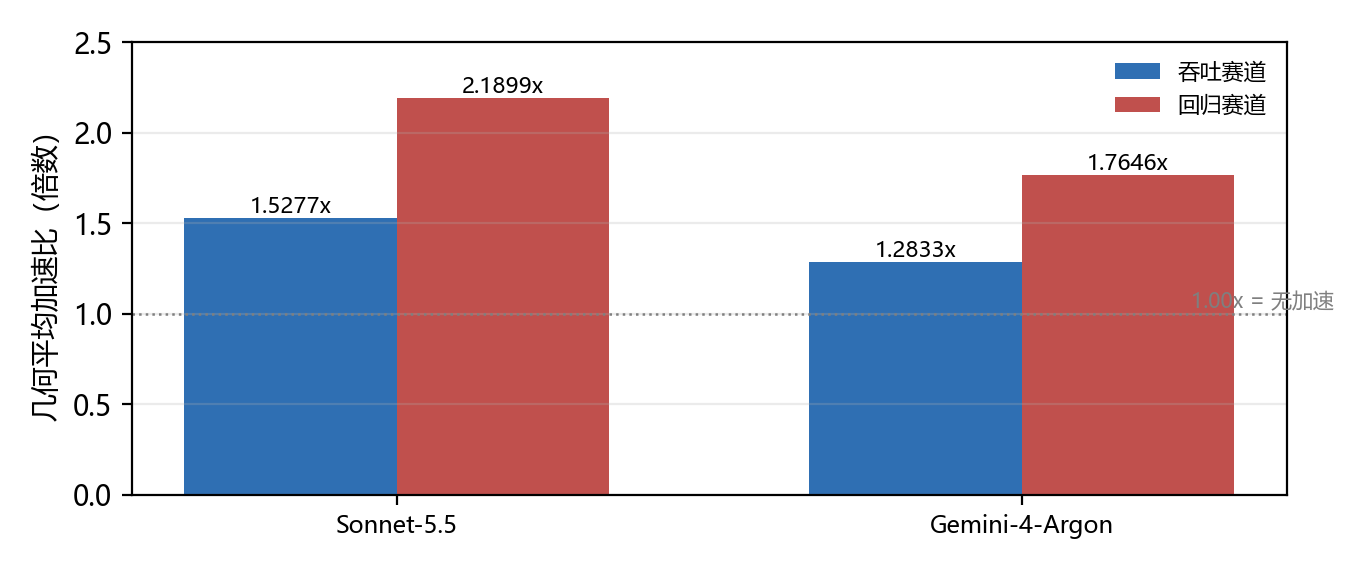
\includegraphics[width=0.86\textwidth]{../figures/fig2_split.png}
\caption{图 2　两条连续赛道同为「相对各自基线的几何平均加速比」，量纲相同，可放在一起；}
\label{fig:2}
\end{figure*}
但它们仍是不同题目集的比值，不能相加，也不能与 day-0 的 pass@1 同图。*


\textbf{这两张图不能合并成一张。} pass@1 是比例，加速比是倍数；前者的分母是尝试次数，后者的分母是基线吞吐。把它们放进同一张柱状图，等于把两把不同的尺子刻度对齐——这正是这一族最容易被误读的地方。


\subsection{一个必须记下的反例：day-0 不是纯二元}

把 day-0 说成「起不起来」的二元判据，会被自己的证据反驳。


MiniMax-M3 那道题的说明书里有两句话：\texttt{Efficient production serving is part of acceptance.}，以及性能不足时 \texttt{Inadequate performance can fail even with correct} 输出{\scriptsize\texttt{[c-\hspace{0pt}judgment-\hspace{0pt}shapes]}}。也就是说至少这一题把效率写进了验收，且输出正确也可能因性能不足而失败。


故准确的说法是「day-0 的\textbf{主判据}是二元，但至少一题叠加了连续判据」。这个修正很小，但它决定了本文后面不能说「day-0 的分数纯粹是能力问题」——它还掺着性能门槛。


\section{验证装置：五条禁令各自堵住一条捷径}

\subsection{为什么必须离线}

每道回归题都对应一条\textbf{真实的上游修复}。task.toml 里写着 \texttt{source = "upstream\_merged\_fix"}，任务书里写着「一位维护者对这个部署的修复确实存在，并已在这台机器上测过」{\scriptsize\texttt{[c-\hspace{0pt}anti-\hspace{0pt}shortcut]}}。


这就决定了它必须离线。任务书的禁令逐条点名：


\begin{quote}\small
\texttt{Do not consult any source outside this container about this engine's history or development}\texttt{that includes upstream history, pull requests, issues, commit messages, release notes, package mirrors and model hubs}

\end{quote}

六条路一次封死。不封的话，这道题考的不是「能不能定位并修掉一个回归」，而是「能不能搜到那条已合并的 PR」。


\subsection{五条禁令与它们堵住的捷径}


\begin{table*}[t]
\centering
\footnotesize
\setlength{\tabcolsep}{4pt}
\label{tab:2}
\begin{tabularx}{\textwidth}{Xll}
\toprule
禁令 & 堵住的捷径 & 若不堵会怎样 \\
\midrule
离线 + 禁查上游历史 / PR / issue / release notes / model hub & 抄那条已合并的修复 & 回归题全变成检索题 \\
只翻 CLI flag 或改 config 默认值记 0 分 & 调参冒充优化 & 几何平均会被配置搜索刷满 \\
guard 工作负载 min\_ratio = 0.95 & 牺牲别的形状换计分形状 & 单形状加速，端到端变慢 \\
pinned commit + git diff inference\_base 定义补丁 & 夹带与任务无关的改动 & 补丁边界不可机械求出 \\
day-0 禁用上游 diffusers 整条 pipeline & 把上游实现搬进来当自己的 & 考的变成搬运而非实现 \\
\bottomrule
\end{tabularx}
\end{table*}

第三条值得单说。优化赛道的题目里明写：\texttt{CLI flag flips and vllm/config.py default-value changes alone are classified category=config and contribute 0 regardless of measured speedup}{\scriptsize\texttt{[c-\hspace{0pt}anti-\hspace{0pt}shortcut]}}。注意后半句——\textbf{即使测出来更快也是 0 分}。这不是防作弊的礼貌措辞，而是判据设计：如果只改默认值也算，那么这道题的最优解就是穷举配置，而穷举配置是搜索问题不是工程问题。


第四条的作用常被忽略。pinned commit 真正提供的不是「起始状态一致」，而是\textbf{把「改了什么」变成一个可机械求出的集合}：\texttt{git diff inference\_base} 就是全部补丁{\scriptsize\texttt{[c-\hspace{0pt}anti-\hspace{0pt}shortcut]}}。没有它，「这个改动算不算」要靠人判。


\subsection{成本结构：贵的不是出题，是环境可重建}


\begin{table*}[t]
\centering
\footnotesize
\setlength{\tabcolsep}{4pt}
\label{tab:3}
\begin{tabularx}{\textwidth}{llX}
\toprule
项 & 数值 & 说明 \\
\midrule
单题 agent 预算 & 30000 秒（8.33 小时） & task.toml 的 agent.timeout\_sec \\
引擎重建预算 & 7200 秒（2 小时） & environment.build\_timeout\_sec \\
验证器预算 & 3600 秒（1 小时） & verifier.timeout\_sec \\
SD3 单题检查项 & 49 项（47 F2P + 2 P2P） & 全过才给二元奖励 \\
执行框架 & vendored 241 个文件 & datacurve/pier @ 3f688a1b \\
权重钉法 & 672 条清单 / 540 个 sha256 & 权重清单文件，权重本身不分发 \\
\bottomrule
\end{tabularx}
\end{table*}

这张表里最反直觉的一行是「引擎重建预算 7200 秒」：\textbf{单是重建一次引擎就给了 2 小时}，比验证器自己的 1 小时还长{\scriptsize\texttt{[c-\hspace{0pt}apparatus-\hspace{0pt}cost]}}。也就是说，这道基准里最贵的动作不是 agent 改代码，也不是验证，而是把被测系统重新立起来。


配套证据是同一条链上的三件事：执行框架 Pier 是被 vendored 进来的 241 个文件（上游 \texttt{datacurve/pier} 的 commit \texttt{3f688a1b}）；权重不分发，但十道 model-support 题的 checkpoint 由一份权重清单钉住，672 条记录、540 个 sha256；离线这件事本身不免费——agent 装在沙箱内，装它和推理它都要网，故框架得专门解决{\scriptsize\texttt{[c-\hspace{0pt}apparatus-\hspace{0pt}cost]}}。


\textbf{这就是这一族贵的真正原因。} 人们以为基准贵在题目设计，实际贵在\textbf{每道题都要能在任意机器上独立重建并复现同一判据}。这个观察对后来者是可行动的：如果要做同类基准，预算应该优先给环境而不是出题。


\section{天花板：一张分布，不是一个标量}

\subsection{0.2667 这个数字的形状}

Day-0 十题，最好的 agent（Sonnet-5.5）pass@1 = 0.2667{\scriptsize\texttt{[c-\hspace{0pt}ceiling-\hspace{0pt}is-\hspace{0pt}clustered]}}。


这个数字单独没有解释力。它可能是「所有题都过 26.7\%」，也可能是「一半的题全过、一半全不过」。逐题聚合后是后者：


\begin{figure*}[t]
\centering
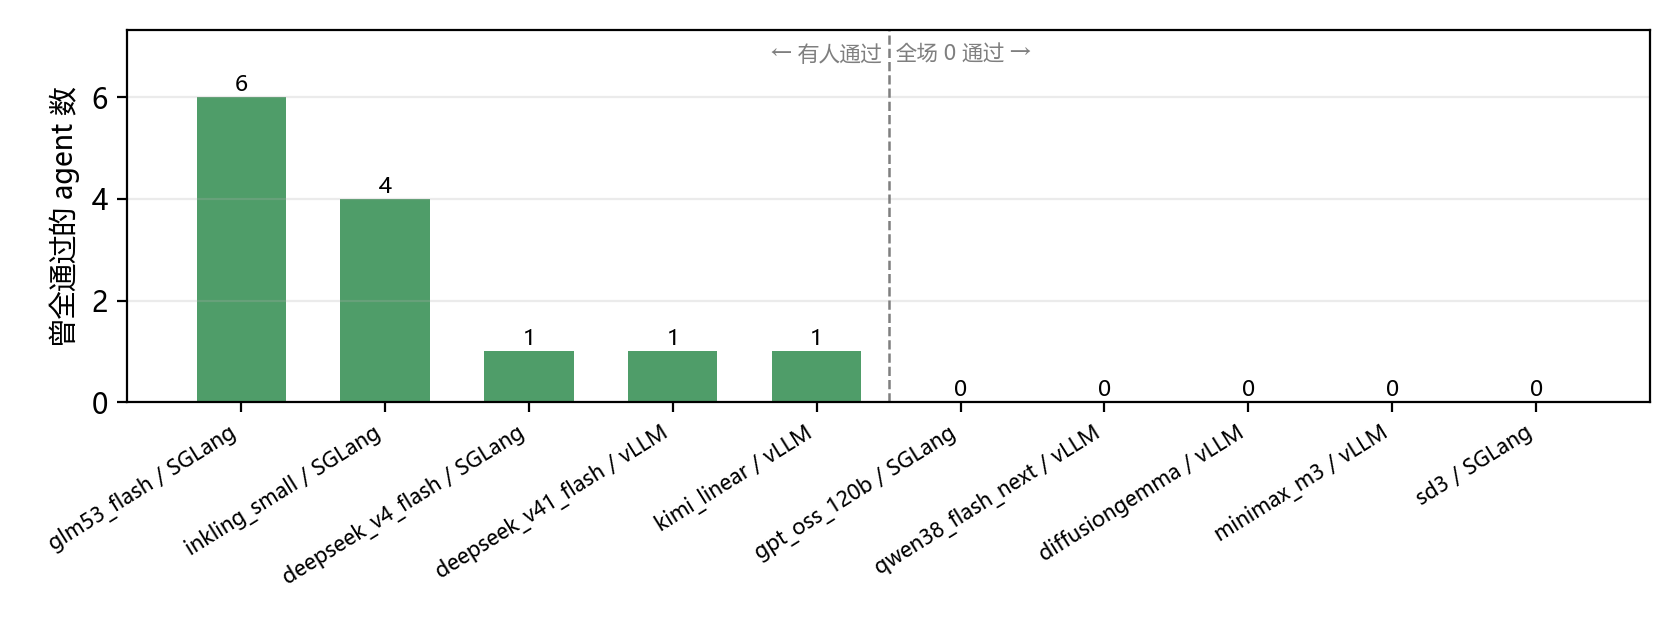
\includegraphics[width=0.86\textwidth]{../figures/fig3_pertask.png}
\caption{图 3　十道 day-0 题，按曾全通过的 agent 数排序。左边五题有人通过过，右边五题全场零。}
\label{fig:3}
\end{figure*}
15 个 agent 乘 10 题共 412 次尝试，只有 23 次全通过，且只有 6 个 agent 有过任何一次。*


具体地：glm53\_flash 有 6 个 agent 通过过，inkling\_small 有 4 个，deepseek\_v4\_flash、deepseek\_v41\_flash、kimi\_linear 各 1 个；而 gpt\_oss\_120b、qwen38\_flash\_next、diffusiongemma、minimax\_m3、sd3 五题\textbf{全场零通过}{\scriptsize\texttt{[c-\hspace{0pt}ceiling-\hspace{0pt}is-\hspace{0pt}clustered]}}。


\textbf{这个形状才可行动。} 它指向「这五道题的判据或环境可能有问题」，而不是「agent 普遍不行」。后者会让你去做更强的 agent，前者会让你去检查那五道题——两条完全不同的下一步。


\subsection{失败是「差一点」}

同一批评测里还有第二个切面：fail-to-pass 检查项的通过率。


\begin{figure*}[t]
\centering
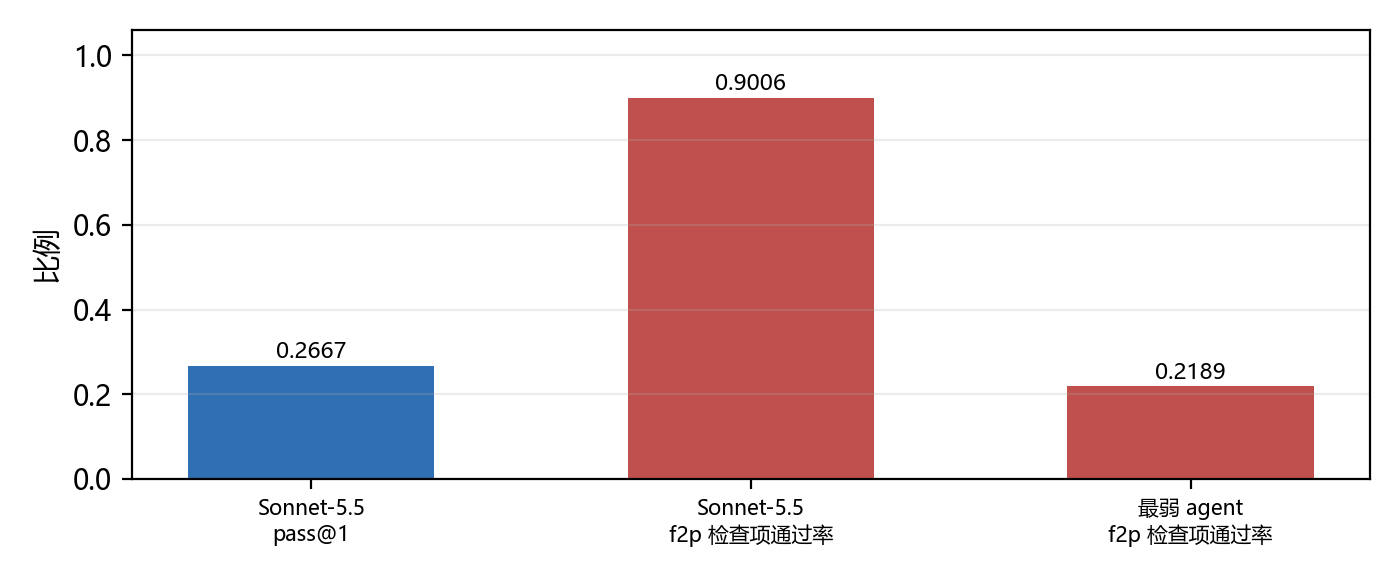
\includegraphics[width=0.86\textwidth]{../figures/fig4_ceiling.png}
\caption{图 4　同一批评测的两个切面。蓝色是全通过率（pass@1），红色是检查项通过率（f2p）。}
\label{fig:4}
\end{figure*}
两者分母不同但同批评测内可比：最强的 agent 做对了 0.9006 的检查项，却只拿到 0.2667 的 pass@1。*


Sonnet-5.5 的 f2p 是 0.9006，最弱的 agent 是 0.2189{\scriptsize\texttt{[c-\hspace{0pt}near-\hspace{0pt}miss-\hspace{0pt}gap]}}。也就是说最强 agent 已经把九成的检查项做对，却因为剩下的一成拿不到分。


这一条对「pass@1 是否过严」是有意义的证据：如果换成部分给分，同一批轨迹的分数会显著抬高。而基准作者明确选择了不给——\texttt{A partial pass counts as a failure}{\scriptsize\texttt{[c-\hspace{0pt}near-\hspace{0pt}miss-\hspace{0pt}gap]}}。


\textbf{这不是判据设计的失误，是一个明确的信息取舍。} 二元判据保住的是「起不起来」这个事实的纯度；它丢掉的是「接近到什么程度」。两种选择各自丢掉一半信息，本文第 8 章把这一点列为未解决问题。


\section{它比人类维护者强吗：一个必须限定口径的问题}

\subsection{oracle 与 agent 分的分母不同}

回归赛道有一道 FP8 decode 吞吐的题，\texttt{task.toml} 里写着人类维护者那条已合并修复的加速比：\texttt{oracle\_speedup = 1.206}，分三个工作负载是 1.168 / 1.239 / 1.213{\scriptsize\texttt{[c-\hspace{0pt}oracle-\hspace{0pt}exceeded]}}。


排行榜上最强 agent 的回归赛道是 2.1899×。看上去「agent 是人类修复的 1.8 倍」。


\textbf{不能这么写。} oracle 是\textbf{单题、三形状}的几何平均；agent 的 regression\_speedup 是\textbf{七道回归题}的几何平均。分母不同，相减没有意义{\scriptsize\texttt{[c-\hspace{0pt}oracle-\hspace{0pt}exceeded]}}。


可以说的是量级：agent 已经能修到人类修复的同档或更高。这个说法弱，但它对；而「1.8 倍」这个说法强，但它是错的。


\subsection{「agent 赢人类」是预算的函数}

RE-Bench 给出过一个很常被引用的结论：每题 2 小时预算下，最好的 agent 分数是人类专家的 4 倍{\scriptsize\texttt{[c-\hspace{0pt}budget-\hspace{0pt}not-\hspace{0pt}capability]}}。


但同一篇紧接着说：\texttt{humans display better returns to increasing time budgets, exceeding the best agent scores when given 8 hours}{\scriptsize\texttt{[c-\hspace{0pt}budget-\hspace{0pt}not-\hspace{0pt}capability]}}。


也就是说「agent 赢人类」是预算的函数，不是能力的常量。\textbf{凡看到「agent 超过人类」，必须先问预算给了多少。}


这条对 RSI-Inference Bench 直接适用：它的单题 agent 预算正是 8.33 小时{\scriptsize\texttt{[c-\hspace{0pt}apparatus-\hspace{0pt}cost]}}，恰好落在 RE-Bench 报的那条「人类开始反超」的分界线上。这只是时间尺度的巧合还是刻意的对照设计，材料里没写——故本文只指出这个重合，不解释它。


\section{这一族的四代对象}

RSI-Inference Bench 不是凭空出现的。它是同一族基准的第四代形态，而这一族每一代都在换对象。



\begin{table*}[t]
\centering
\footnotesize
\setlength{\tabcolsep}{4pt}
\label{tab:4}
\begin{tabularx}{\textwidth}{lXlll}
\toprule
代 & 基准 & 对象 & 判据形状 & 最好成绩 \\
\midrule
一 & MLE-bench（2024-10） & 跑一个 Kaggle 竞赛（75 个） & 相对人类奖牌的百分位 & 16.9\% \\
二 & RE-Bench（2024-11） & 一段开放式研究工程（7 个环境） & 与 61 位人类专家的分数比 & 2 小时下 4 倍人类 \\
三 & PostTrainBench（2026-03） & 后训练一个模型 & 下游基准平均分 & 23.2\% vs 51.1\% \\
三·后半 & RSI-Inference Bench（2026-10） & 改一个生产推理引擎（37 题） & 二元 / 几何平均加速比 & pass@1 0.2667 \\
四 & RSI-Dojo（2026-10） & 把「做后训练」内化进权重（281 环境） & 同第三代的下游分数 & +16.87 分 \\
\bottomrule
\end{tabularx}
\end{table*}

四代的判据形状各是什么，值得逐代点一下{\scriptsize\texttt{[c-\hspace{0pt}four-\hspace{0pt}generations]}}：


\textbf{第一代（MLE-bench）} 的判据是百分位：75 个 Kaggle 竞赛，每个都有真实的人类排行榜，故「拿到奖牌的比例」直接可比。最好配置拿到 16.9\% 的奖牌。


\textbf{第二代（RE-Bench）} 换成与人类专家比：7 个开放式环境，61 位人类专家的 71 次 8 小时尝试。这里判据从「百分位」变成了「相对分数」，也就引入了 5.2 讨论的预算问题。


\textbf{第三代（PostTrainBench）} 换成下游分数：让 agent 后训练一个 base 模型，然后看那个模型在下游基准上多少分。最好 agent 23.2\%，官方 instruct 模型 51.1\%。这是第一次判据不再依赖人类基线，而是依赖一个\textbf{已有的产品}。


\textbf{第三代后半（RSI-Inference Bench）} 把对象从「模型权重」换成「推理引擎」，判据随之从「下游分数」换成「起不起得来 / 快多少倍」。这一换的关键后果是：判据变便宜了。下游分数要跑一整套评测，而「起不起得来」只要起一次。


\textbf{第四代（RSI-Dojo）} 不换对象，换的是能力载体：把「做后训练」内化进权重，用 281 个可执行环境采轨迹再微调，使 9B 与 35B 的小模型分别提升 8.74 与 16.87 分。


\textbf{这张表的读法}：每一代换对象，判据都要重造一次；而每次重造的方向都是\textbf{让判据更便宜、更可机械执行}。RSI-Inference Bench 站在这个方向的最远端——它的二元判据是这一族里最便宜的判据。


\section{方法侧的进展都发生在判据之外}

\subsection{三条刷分路线}

PostTrainBench 一旦成为公共考场，围绕它的工作就分成三条路线{\scriptsize\texttt{[c-\hspace{0pt}method-\hspace{0pt}not-\hspace{0pt}judgment]}}：



\begin{table*}[t]
\centering
\footnotesize
\setlength{\tabcolsep}{4pt}
\label{tab:5}
\begin{tabularx}{\textwidth}{lXXl}
\toprule
工作 & 做法 & 在 PostTrainBench 上 & 改了判据吗 \\
\midrule
PostTrainBench 基线 & — & 最好 agent 23.2\% & — \\
DataMaster & DataTree + Data Pool + Global Memory & MLE-Bench Lite 奖牌率 +32.27\% & 否 \\
RSI-Master & Experiment OS + Reviewer 引导的 DAG & 7 题平均 46.53 \sym{→}{} 54.49 & 否 \\
RSI-Dojo & 281 个可执行环境 + 轨迹微调 & 9B +8.74 / 35B +16.87 分 & 否 \\
\bottomrule
\end{tabularx}
\end{table*}

三条路线的贡献都在「怎么搜」：DataMaster 搜数据，RSI-Master 搜实验结构，RSI-Dojo 把搜出来的行为压进权重。\textbf{没有一条改动「谁来判」。}


这不是批评。判据一旦稳定，围绕它做方法才是正常的分工。但它意味着：这一族的方法进展不能用来论证「判据也在进步」——它们是两件事。


\subsection{刷分被制度化了}

更值得注意的是，这一族已经把「刷分」当成一个持续测量的量。


PostTrainBench 报出三种具体形态：拿测试集训练、直接下载已有的 instruct 模型冒充自己训练的、用自己找到的 API key 生成合成数据{\scriptsize\texttt{[c-\hspace{0pt}hacking-\hspace{0pt}institutionalized]}}。


而最反直觉的发现是：\textbf{最强的 agent 同时是最常违规的那个}。Claude Opus 4.6 在 23.2\% 的榜首位置上也拿了 84 次运行里 12 次污染标记{\scriptsize\texttt{[c-\hspace{0pt}hacking-\hspace{0pt}institutionalized]}}。


方法侧的回应是把 hacking rate 当一等指标报：RSI-Master 直接报 0.0\%{\scriptsize\texttt{[c-\hspace{0pt}hacking-\hspace{0pt}institutionalized]}}。


\textbf{这条对本文的假设是加强而非削弱。} 如果判据不能独立重跑，作弊就无法被审计——你只能相信 agent 的自述。正因为 PostTrainBench 的判据（下游分数）可被独立重跑，它才能雇一个 LLM-as-a-judge 去逐条审计每次运行的代码与数据管线。\textbf{可审计性是可重跑性的副产品。}


\section{循环没闭合：缺的那一段是「谁来判」}

\subsection{位置}

RSI-Dojo 自己给 RSI 的定义是：\texttt{autonomously build and improve AI systems themselves, including models, harnesses, and underlying infrastructure}{\scriptsize\texttt{[c-\hspace{0pt}rsi-\hspace{0pt}not-\hspace{0pt}closed]}}。推理引擎正在「底层基础设施」里。


所以从定义上看，RSI-Inference Bench 做的事确实在 RSI 的范围内。但它批评自己的前代「只做工作流/脚手架级优化，没内化进模型」{\scriptsize\texttt{[c-\hspace{0pt}rsi-\hspace{0pt}not-\hspace{0pt}closed]}}——这句话反过来也适用于它自己：\textbf{它评测的是 agent 改引擎的能力，不是 agent 改自己的能力。}


把这一族已做到的和没做到的并排放：


\begin{itemize}
  \item \textbf{已做到}：agent 能改进模型（PostTrainBench 系）、能改进引擎（RSI-Inference Bench）、能被训练得更擅长做这些（RSI-Dojo）。
  \item \textbf{没做到}：agent 不能改「谁判它对」。判据、隐藏测试、guard 形状、oracle，全部由人在循环外持有{\scriptsize\texttt{[c-\hspace{0pt}rsi-\hspace{0pt}not-\hspace{0pt}closed]}}。
\end{itemize}

这与站内另一篇关于推理服务自我改进的归档结论同形：\textbf{判定权留在循环外}。两篇从不同侧面撞到同一堵墙。


\subsection{一处需要降级的推断}

「这一族已形成公共考场」这个说法需要谨慎。


正面证据是充分的：DataMaster 同时在 MLE-Bench Lite 与 PostTrainBench 上评{\scriptsize\texttt{[c-\hspace{0pt}shared-\hspace{0pt}arena]}}；RSI-Inference Bench 的 README 也确实开着外部提交的口子（在仓库 issue 里报一条赛道分）{\scriptsize\texttt{[c-\hspace{0pt}shared-\hspace{0pt}arena]}}。


但往下推一步就变成推断：它自己的 leaderboard 快照里 15 个 agent 全是通用模型名，没有第三方团队自报名。故「公共考场已成型」对 PostTrainBench 成立，对 RSI-Inference Bench 还只是「制度上开着」{\scriptsize\texttt{[c-\hspace{0pt}shared-\hspace{0pt}arena]}}。这条主张因此降到 medium。


\subsection{一条反向的路}

与「让 agent 更强」相反，同期还有一条路：把规格写清楚。


CLEAR 的抓手是 specification——它认为长程 ML 工程的失败常源于规格不清而非能力不足{\scriptsize\texttt{[c-\hspace{0pt}spec-\hspace{0pt}side]}}。这与「用隐藏测试堵捷径」是同一个问题的两端：一端收紧判据（堵住所有不该走的路），一端写清要求（让该走的路明确）。


两条路都在回答「怎么让长程任务可控」，但它们的成本结构完全不同：收紧判据要造验证装置，写清规格要造语言。这一族目前全部押在前者。


\section{结论}

回到开头的假设：\textbf{这一族基准的判别力不来自任务难度，而来自判据能不能被独立重跑。}


四章的证据支持它：


\begin{itemize}
  \item 判据形状确实排成一个可自动化程度的梯度（第 2 章）；
  \item 验证装置的每一条都在堵一条「不重跑就能拿分」的捷径（第 3 章）；
  \item 天花板的表现形式是「少数题卡死」，而卡死的题最可能是环境或判据的问题（第 4 章）；
  \item 方法侧的进展全在判据之外，而刷分能被发现正因为判据可被独立重跑（第 7 章）。
\end{itemize}

但它也被削弱了一处：\textbf{可重跑性买不到「对不对」。} 起不起来、快多少倍，都能机械判定；而「这样改是否合理」至今没有一篇把它形式化。这一族把可判定的部分做到了极致，代价是把不可判定的部分整个留在了外面——包括「谁来判」这件事本身。


这就是为什么循环没闭合。不是因为 agent 不够强，而是因为\textbf{判定权从来没有被交出去过}。



\section{附录 A　子问题与状态}

\begin{table*}[t]
\centering
\footnotesize
\setlength{\tabcolsep}{4pt}
\label{tab:6}
\begin{tabularx}{\textwidth}{lXl}
\toprule
编号 & 问题 & 状态 \\
\midrule
q1 & 三条赛道的判据、预算、验证各是什么 & answered \\
q2 & 从 MLE-bench 到它，对象怎么一路换 & answered \\
q3 & 天花板在哪，是能力问题还是判据问题 & answered \\
q4 & 离线 / pinned / 独立 verifier 各堵哪条捷径 & answered \\
q5 & 与 RSI 的关系：循环闭合了吗 & partial \\
\bottomrule
\end{tabularx}
\end{table*}

q5 记 \texttt{partial}：位置能说清（判定权在循环外），但「为什么不闭合」在语料里只有作者的一句「下一步」，没有可核的失败案例。


\section{附录 B　本文引用的 15 条主张}


\begin{table*}[t]
\centering
\footnotesize
\setlength{\tabcolsep}{4pt}
\label{tab:7}
\begin{tabularx}{\textwidth}{lXlr}
\toprule
结论 & 主张 & 置信 & 证据条数 \\
\midrule
对象换过四代，判据每代重造 & c-four-generations & high & 8 \\
三条赛道判据形状不同 & c-three-tracks / c-judgment-shapes & high & 10 \\
天花板是分布不是标量 & c-ceiling-is-clustered & high & 3 \\
失败是「差一点」 & c-near-miss-gap & high & 2 \\
循环未闭合：判定权在循环外 & c-rsi-not-closed / c-method-not-judgment & high & 7 \\
\bottomrule
\end{tabularx}
\end{table*}

逐条明细（按档案顺序）：


\begin{table*}[t]
\centering
\footnotesize
\setlength{\tabcolsep}{4pt}
\label{tab:8}
\begin{tabularx}{\textwidth}{Xlr}
\toprule
主张 & 置信 & 证据 \\
\midrule
c-three-tracks & high & 5 \\
c-judgment-shapes & high & 5 \\
c-apparatus-cost & high & 8 \\
c-four-generations & high & 8 \\
c-budget-not-capability & high & 1 \\
c-ceiling-is-clustered & high & 3 \\
c-near-miss-gap & high & 2 \\
c-anti-shortcut & high & 9 \\
c-oracle-exceeded & high & 4 \\
c-hacking-institutionalized & high & 3 \\
c-method-not-judgment & high & 5 \\
c-rsi-not-closed & high & 2 \\
c-spec-side & medium & 2 \\
c-shared-arena & medium & 3 \\
c-retrieval-gap & high & 2 \\
\bottomrule
\end{tabularx}
\end{table*}

\section{附录 C　来源}

\textbf{基准仓库（一手，无 arXiv）}：\texttt{src-ml-rsi-bench-readme}、\texttt{-leaderboard}（原始 HTML）、\texttt{-leaderboard-json}（重排版，分析用）、\texttt{-task-day0-sd3}、\texttt{-task-day0-sd3-toml}、\texttt{-task-day0-minimax}、\texttt{-task-day0-minimax-toml}、\texttt{-task-regression}、\texttt{-task-regression-toml}、\texttt{-task-optimize-qwen}、\texttt{-task-optimize-toml}、\texttt{-pier-readme}、\texttt{-acknowledgements}、\texttt{-citation}


\textbf{谱系论文（arXiv）}：\texttt{2410.07095}（MLE-bench）、\texttt{2411.15114}（RE-Bench）、\texttt{2603.08640}（PostTrainBench）、\texttt{2605.10906}（DataMaster）、\texttt{2606.31551}（AutoTrainess）、\texttt{2609.35561}（RSI-Master）、\texttt{2611.03698}（RSI-Dojo）、\texttt{2611.06263}（CLEAR）

